\section{Context-dependency model to WFST}
\label{sec:cdmod}

\subsection{Sub-word Units}
\label{sec:subword}
The context dependency model maps sequences of context dependency phones (the sub-word units presented in a GMM based acoustic model) to sequences of monophones (the sub-word units used in a pronunciation model).

There are two variants of context-dependency models using different strategies to cope with \textit{word boundary} information. One is word-internal model, and the other is cross-word model. The example below shows the differences of these two methods. 

For simplicity, we will focus on the cross-word context dependency model in subsequent discussions. \vspace{5mm}

\textbf{Word-internal} context dependency:

Word boundaries represent a distinct context.
\begin{Verbatim}[frame=leftline, framesep=5mm]
speech task =
/sil s+p s-p+iy p-iy+ch iy-ch
t+ae t-ae+s ae-s+k s-k sil/
\end{Verbatim}

\textbf{Cross-word} context dependency:

Word boundaries are ignored or used as additional context information.
\begin{Verbatim}[frame=leftline, framesep=5mm]
speech task = 
/sil sil-s+p s-p+iy p-iy+ch iy-ch+t
ch-t+ae t-ae+s ae-s+k s-k+sil sil/
\end{Verbatim}

\subsection{Basic Representation} 
\label{cdrep}

Basically, the C WFST is constructed by the rules~\cite{dixonintroduction} stated in Table~\ref{tbl:cdrules}.
 
\begin{table}[H]
\begin{center}
  \begin{tabular}{| c | c | c | c | c |}
  \hline
  Type & Source & Destination & Input Symbol & Output Symbol \\ \hline
  l-c+r & l,c & c,r & l-c+r & r \\ \hline
  c+r & -,c & c,r & c+r & r \\ \hline
  l-c & l,c & c,-(Final) & l-c & - \\ \hline
  c & -,-(Start) & -,c & - & c \\ \hline
  c & -,c & c,-(Final) & c & - \\ \hline
  \end{tabular}
  \caption{Context dependency model to WFST construction rules}
  \label{tbl:cdrules}
\end{center}
\end{table}

Figure~\ref{c_prototype} shows a prototype C WFST, the context independent phones are $x$ and $y$ only.

\begin{figure}[H]
  \centering
  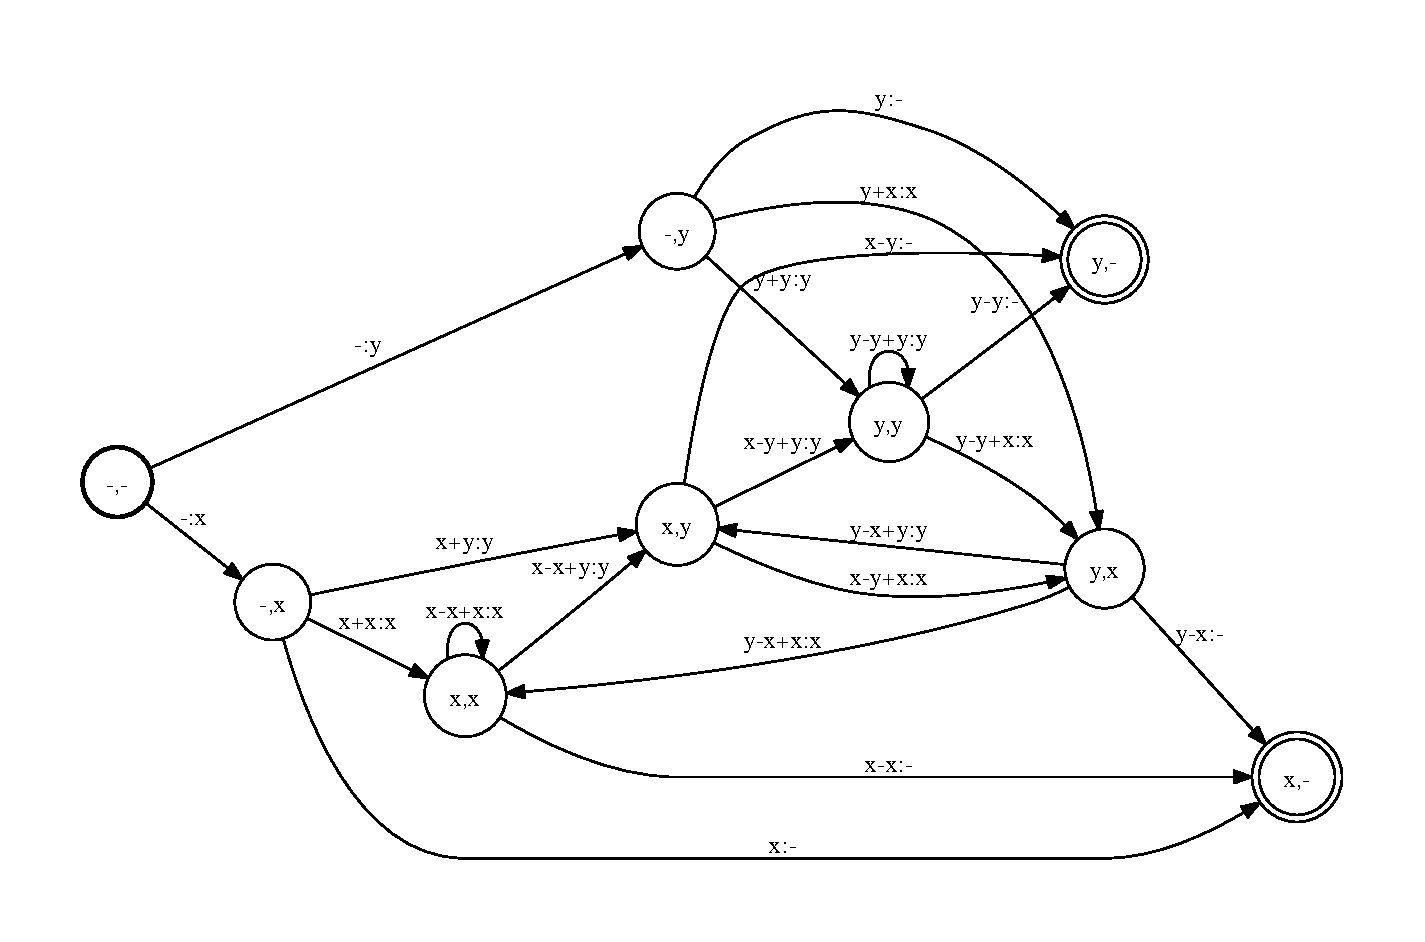
\includegraphics[width=0.7\textwidth]{./figures/c_prototype.pdf}
  \caption{A prototype C WFST}
  \label{c_prototype}
\end{figure}

There is a very small emparical C WFST constructed by Juicer (cdgen) depicted in Figure~\ref{c_no_sp_aux}. Notice that we assume that all logical triphones are physical triphones. We use only one silence model ``sil'' and the auxiliary symbols are not illustrated. All triphones in tiedlist are in set $\{sil\}\cup\{f,uw,sil\}\times\{f,uw\}\times\{f,uw,sil\}$.

\begin{figure}[H]
  \centering
  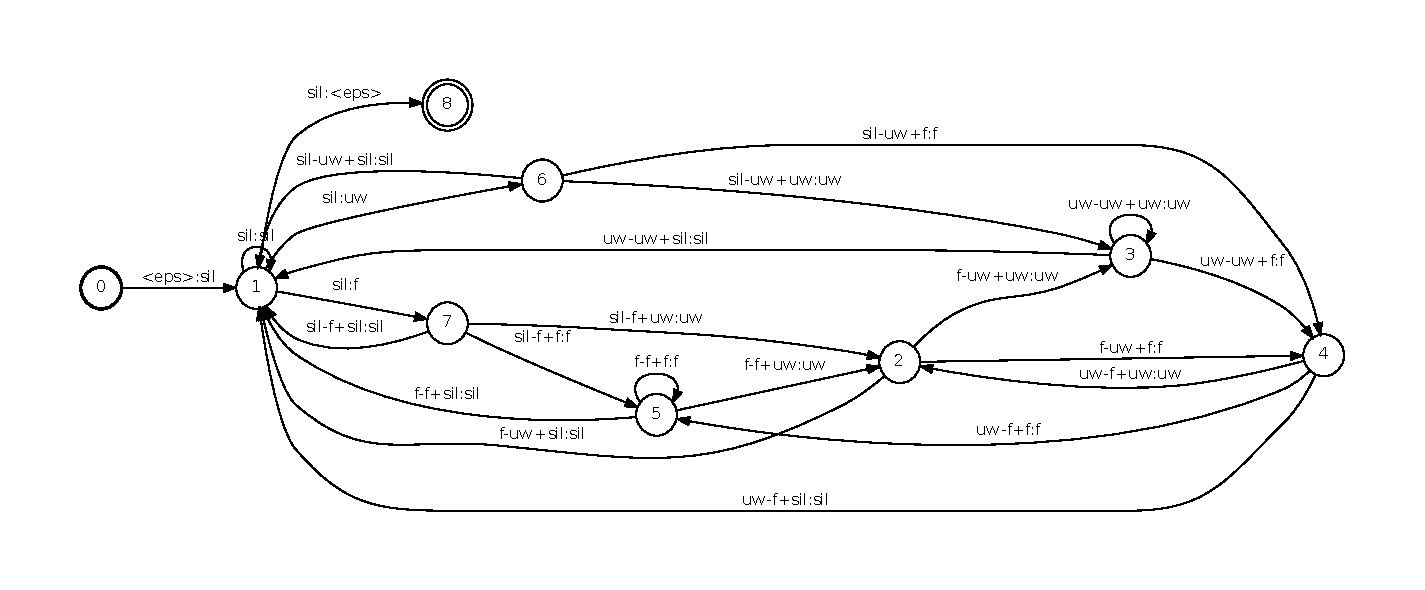
\includegraphics[width=\textwidth]{./figures/c_no_sp_aux.pdf}
  \caption{A simple cross-word type C WFST}
  \label{c_no_sp_aux}
\end{figure}

\subsection{Silence Modeling}
\label{silmod}
There are two silence models described and advocated to use in acoustic model by Young, \textit{et al}~\cite{young2006htk}. 

\begin{itemize}
\item
  A silence model, \texttt{sil}, with the same structure as the other phonetic models, acts as a context, but is context dependent.
\item
  A short pause model, \texttt{sp}, is tied to the silence model. Short pause model is context free.
\end{itemize}

\subsubsection{Silence Modeling in Juicer}
\label{juicer_sil}

There are two different routines to apply short pause model in C WFST described by Garner \textit{et al}~\cite{garner2008silence}. The insertion of \texttt{sp} into transitions in C is illustrated in Figure~\ref{c_sp_model}.

\begin{figure}[!ht] 
  \centering
  \subfloat[Juicer's implementation]{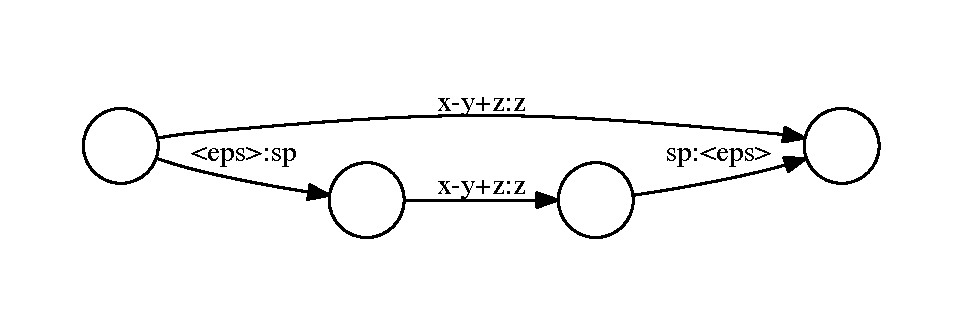
\includegraphics[width=0.6\textwidth]{./figures/c_sp1.pdf}} ~
  \subfloat[A more compact form]{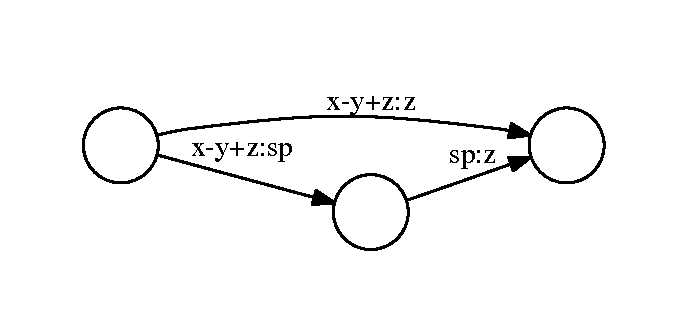
\includegraphics[width=0.4\textwidth]{./figures/c_sp2.pdf}} ~
  \caption{Insertion of \texttt{sp} into transitions in C}
  \label{c_sp_model}
\end{figure}

To accommodate silence at the lexicon level, the insertion of \texttt{sp} into transitions in L is also needed. Figure~\ref{l_sil_sp} shows the three pronounciations of a single word \texttt{NO}.

\begin{figure}[H]
  \centering
  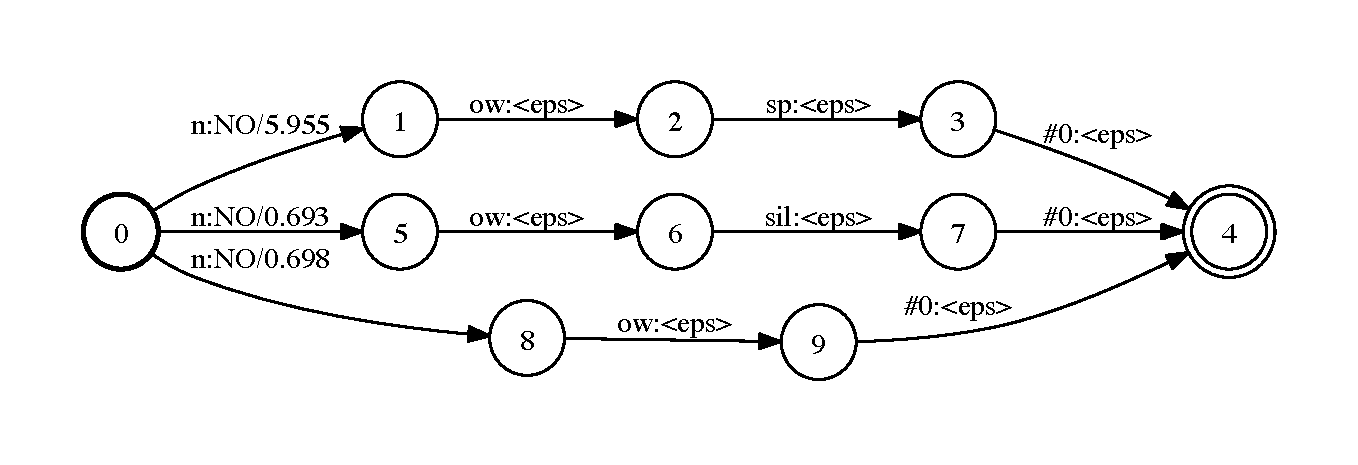
\includegraphics[width=0.8\textwidth]{./figures/l_sil_sp.pdf}
  \caption{An example of L WFST with silence phones}
  \label{l_sil_sp}
\end{figure}

\subsubsection{Silence Modeling in Transducersaurus}
\label{josef_sil}
In Transducersaurus' implementation, a silence transducer T is introduced. Thus the traditional C$\circ{}$L$\circ{}$G composition is modified to C$\circ{}$L$\circ{}$G$\circ{}$T. With this approach, silences are treated as just like other words, as described in~\cite{allauzen2004generalized}. Figure~\ref{silcls} shows the basic representation of a silence transducer T. To allow more complex silence modeling, class-based approach can be applied in transducer T. But currently only the silence transducer in Figure~\ref{silcls} is implemented.

\begin{figure}[H]
  \centering
  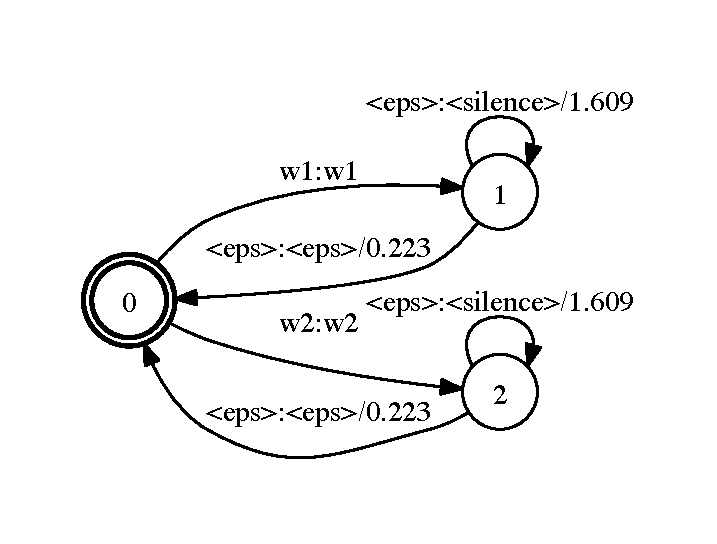
\includegraphics[width=0.5\textwidth]{./figures/silcls.pdf}
  \caption{A simple silence transducer T}
  \label{silcls}
\end{figure}

\subsection{Auxiliary Symbols}
\label{cdaux}
If the auxiliary labels are left in L$\circ$G, then C WFST must add some auxiliary transitions to match those in L$\circ$G. The easiest way to implement is to add auxiliary loops on all states of C WFST, as illustrated in Figure~\ref{c_aux}. 

\begin{figure}[H]
  \centering
  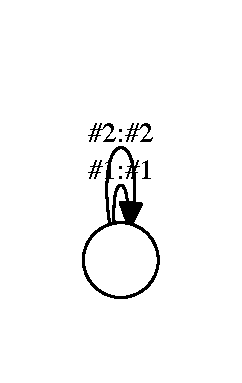
\includegraphics[width=0.2\textwidth]{./figures/c_aux.pdf}
  \caption{Auxiliary loops on states of C WFST}
  \label{c_aux}
\end{figure}